% -*- root: ../Thesis.tex -*-
\chapter{Modelowanie przestrzenne}
\label{chap:modelowaniePrzestrzenne}
\section{Równania reakcji-dyfuzji w~modelach ciągłych} 
%%%%%%%%%%%%%%%%%%%%%%%%%%%%%%%%%%%%%%%%%%%%%%%%%%%%%%%%%%%%%%%%%%%%%%%%%%%%%%%%%%%%%%%%%%%%%%%%%%%%%%%
%%%%%%%%%%%%%%%%%%%%%%%%%%%%%%%%%%%%%%%%%%%%%%%%%%%%%%%%%%%%%%%%%%%%%%%%%%%%%%%%%%%%%%%%%%%%%%%%%%%%%%%
Najprostszy przestrzenny model dynamiki wapnia w komórce zadany jest przez jedno równanie typu reakcji-dyfuzji na stężenie jonów wapniowych 
w cytozolu: 

\begin{equation} \label{stand} \dfrac{\p c(x,t)}{\p t} = D \Delta c(x,t) + f(c(x,t))
\end{equation} 

\noindent W równaniu powyższym $c=c(x,t)$ oznacza stężenie niezwiązanych jonów wapnia w~punkcie $x \in \Omega$ i czasie $t \geq 0$. $\Omega$ \textit{jest tutaj otwartym (i prezwartym) obszarem modelującym rozpatrywany obszar komórki}, $f(c)$ jest funkcją charakteryzującą przepływ wapnia między cytozolem a zewnętrzem komórki oraz wewnątrzkomórkowymi magazynami wapniowymi. 

\medskip

%%%%%%%%%%%%%%%%%%%%%%%%%%%%%%%%%%%%%%%%%%%%%%%%%%%%%%%%%%%%%%%%%%%%%%%%%%%%%%%%%%%%%%%%%%%%%%%%%%%%%%%%%%%%%%%%%%%%%

W modelu zadanym równaniem (\ref{stand}) zaniedbujemy również procesy przyłączania wapnia przez molekuły buforujące. Uwzględnienie tego zjawiska prowadzi do układu równań na ewolucję stężenia wapnia w cytozolu $c$, 
stężenie molekuł buforujących, które przyłączyły wapń $b_i = [Ca^{2+}\,B_i]$ oraz 
stężenie samych molekuł buforujących $B_i$, które nie przyłączyły jonów wapnia. 
Układ ten ma następującą postać: 


\begin{equation} \label{b1p}
\begin{array}{l}
	{\displaystyle
		\frac{\p c}{\p t} = D_c \Delta c +
		\sum_{i=1}^n [ k^{-}_i b_i - k^{+}_i c B_i] + f(c)
	}\\[2ex]
	{\displaystyle
		\frac{\p {b}_i}{\p t} = D_i \Delta b_i
		- [k^{-}_i b_i - k^{+}_i c B_i], \quad i=1,\ldots,n \geq 1 
	}\\[2ex]
	{\displaystyle
		\frac{\p {B}_i}{\p t} = D_{Bi} \Delta B_i
		+ [k^{-}_i b_i - k^{+}_i c B_i], \quad i=1,\ldots,n \geq 1.
	}
\end{array}
\end{equation}

\noindent Stałe $k^{-}_i>0, k^{+}_i>0$ oznaczają tutaj współczynniki kinetyczne 
odłączania i przyłączania jonów wapnia, $D_c$ jest współczynnikiem dyfuzji dla wolnych jonów wapnia, $D_i$ współczynnikiem dyfuzji dla ,,uwapniowanych'' buforów $i$-tego rodzaju a 
$D_{B_i}$ współczynnikiem dyfuzji dla molekuł buforujących $i$-tego rodzaju. 

\medskip 

Naturalnym, powszechnie czynionym założeniem, jest założenie o równości współczynników dyfuzji 
$D{i}$ oraz $D_{Bi}$. W tym przypadku łatwo dowieść (poprzez dodanie 
równań na $b_i$ oraz $B_i$), że jeśli w chwili początkowej $t=0$ 
stężenie całkowite molekuł buforujących $i$-tego rodzaju $b_i(x,0) + B_i(x,0)$ jest jednorodne przestrzennie, 
to pozostanie takie również dla wszystkich czasów $t>0$. Tak więc ~$b_i(x,t) + B_i(x,t)=b^i_0= const$, 
$b^i_0$ oznacza tutaj całkowite stężenie $i$-tego rodzaju molekuł buforujących, tzn. $b^i_0 =[B_i] + [Ca^{++}\,B_i]$. 
W tym przypadku $B_i(x,t)=b^i_0 - b_i(x,t)$ i możemy ograniczyć się do układu postaci: 



\begin{equation} \label{b1}
\begin{array}{l}
	{\displaystyle
		\frac{\p c}{\p t} = D_c \Delta c +
		\sum_{i=1}^n [ k^{-}_i b_i - k^{+}_i c (b_i^0 -b_i)] + f(c)
	}\\[2ex]
	{\displaystyle
		\frac{\p {b}_i}{\p t} = D_i \Delta b_i
		- [k^{-}_i b_i - k^{+}_i c (b_i^0 -b_i)], \quad i=1,\ldots,n \geq 1. 
	}
\end{array}
\end{equation}

\medskip 

\noindent \textbf{Uwaga}\\\noindent W istocie rzeczy, wskaźnik $i$ w równaniach (\ref{b1}) powinien numerować raczej miejsca wiązania wapnia, np. miejsca typu EF-hand, a nie poszczególne rodzaje molekuł buforujących. Tak więc, jednemu rodzajowi molekuł buforujących powinna odpowiadać liczba wskaźników równa liczbie miejsc typu EF-hand w molekule. Jeśli jednak przy-łączaniekolejnych jonów wapnia nie zmienia istotnie fizycznych własności molekuły, w~szczególności jej współczynnika dyfuzji, to opis dany układem (\ref{b1}) jest wystarczający. \B 

\bigskip 

Bardziej złożonym i dokładnym opisem jest model, w którym podobnie do ,,cytozolicznego'' rozważa się trzy kompartmenty komórkowe: cytozol, retikulum oraz kompartment mitochondrialny. 

\medskip 

Niech $\Omega_{Cyt}, \, \Omega_{Ret}$ oraz $\Omega_{Mit}$ oznaczają podobszary komórki odpowiadające powyższym kompartmentom. Tak więc 

\[ \Omega_{Cyt}, \, \Omega_{Ret}, \, \Omega_{Mit} \subset \Omega \] 

\noindent Zakładamy również, że zbiory $\Omega_{Ret}$ oraz $\Omega_{Mit}$ są rozłączne - 
$\overline{\Omega}_{Ret} \cap \overline{\Omega}_{Mit} = \emptyset$ oraz, że 
$\p \Omega \cap (\p \Omega_{Ret} \cup \p \Omega_{Mit}) = \emptyset$, tzn. że 
organelle retikularne i mitochondrialne są odseparowane od membrany komórkowej. (Ostatnie założenie jest nie do końca słuszne z~uwagi na istnienie obszarów bezpośredniej bliskości obszarów retikularnych i membrany komórkowej). Oczywiście, z racji swojej struktury geometrycznej, zbiory $\Omega_{Ret}, \, \Omega_{Mit}$ mogą być w ogólności zbiorami \textbf{niejednospójnymi}. 

Przyjmujemy, że w kompartmencie $\Omega_\gamma$, $\gamma \in \{{Cyt},\,{Ret},{Mit}\}$, dynamika wapnia dana jest poprzez równania analogiczne do układu (\ref{b1}), tj.

\begin{equation} \label{cga}
{\displaystyle
	\frac{\p c_\gamma}{\p t} = D_c \Delta c_\gamma + \phi(c) \delta_{\gamma;Cyt} + 
	\sum_{i=1}^n [ k^{-}_{i\gamma} b_{i\gamma} - k^{+}_{i\gamma} c (b^0_{i\gamma} -b_{i\gamma})]
}
\end{equation}
\begin{equation} \label{bga}
{\displaystyle
	\frac{\p {b}_{i\gamma}}{\p t} = D_{i\gamma}  \Delta b_{i\gamma} 
	- [k^{-}_{i\gamma} b_{i\gamma} - k^{+}_{i\gamma} c (b^0_{i\gamma} -b_{i\gamma})], \quad i=1,\ldots,n_\gamma \geq 1
}
\end{equation}

\noindent W powyższym układzie $\phi(c)$ oznacza możliwe strumienie jonów wapniowych między wnętrzem komórki a przestrzenią miedzykomórkową, gdzie $\delta_{\gamma;Cyt}$ oznacza deltę Kroneckera (równą $1$ dla $\gamma=Cyt$ oraz $0$ w przeciwnym przypadku). Układ powyższy uzupełniony jest wyrażeniami na dyfuzyjne prądy miedzykompartmentalne, dokładniej $\Phi_{Ret-Cyt}$ pomiędzy retikulum a cytozolem oraz $\Phi_{Mit-Cyt}$ pomiędzy mitochondriami a~cytozolem. Tak więc, układ (\ref{cga})-(\ref{bga}) uzupełniamy na granicach cytozolicznych warunkami typu Robina postaci: 

\begin{equation} \label{RCW}
D_c \boldsymbol{n}(x) \cdot \nabla c(x,t) = \Phi_{Ret-Cyt}(x,t) \quad {\mathrm na} ~~ \Gamma_{Ret-Cyt} 
\end{equation}

\noindent oraz 

\begin{equation} \label{MCW}
D_c \boldsymbol{n}(x) \cdot \nabla c(x,t) = \Phi_{Mit-Cyt}(x,t) \quad {\mathrm na} ~~ \Gamma_{Mit-Cyt} 
\end{equation} 

\noindent oraz warunkami wyrażającymi fakt, że molekuły buforujące (z przyłączonymi jonami wapnia) nie przechodzą przez błony rozgraniczające, tzn. dla $i=1,\ldots,n_{Cyt}$

\begin{equation} \label{RBW}
D_{iRet} \boldsymbol{n}(x) \cdot \nabla b_{iCyt}(x,t) = 0 \quad {\mathrm na}~~ \Gamma_{Ret-Cyt} 
\end{equation}

\noindent oraz dla $i=1,\ldots,n_{Mit}$ 

\begin{equation} \label{MBW}
D_{iMit} \boldsymbol{n}(x) \cdot \nabla b_{iMit}(x,t) = 0 \quad {\mathrm na}~~ \Gamma_{Mit-Cyt} 
\end{equation} 

\medskip 

\noindent gdzie $\Gamma_{Ret-Cyt}$ oznacza zbiór granic cytozoliczno-retikularnych a $\Gamma_{Mit-Cyt}$ oznacza zbiór granic cytozoliczno-mitochondrialnych. $\textbf{n}(x)$ jest tutaj wektorem normalnym do granicy w punkcie $x$ skierowanym w stronę zewnętrzną, tzn. ,,od cytozolu'', $\nabla$ jest operatorem gradientu. Tak więc $\textbf{n}(x) \cdot \nabla$ jest pochodną wzdłuż wektora prostopadłego do granicy skierowanego od kompartmentu cytozolicznego. Przy tej konwencji\\ \mbox{$\Phi_{Ret-Cyt}(x,t)>0$} oznacza, że przepływ jonów wapniowych następuje od retikulum do cytozolu a \mbox{$\Phi_{Mit-Cyt}(x,t)>0$} oznacza, że przepływ jonów wapniowych następuje od mitochondrium do cytozolu w punkcie $x$ rozpatrywanej granicy oraz czasie $t$. Faktycznie, zakłada się, że $\Phi_{Ret-Cyt}(x,t)$ zależy (w sposób algebraiczny) od wartości stężeń $c_{Cyt}(x,t)$ oraz $c_{Ret}(x,t)$ po obu stronach granicy $\Gamma_{Ret-Cyt}$:

\[
\Phi_{Ret-Cyt}(x,t) = \Phi_{Ret-Cyt}\left(c_{Cyt}(x,t),c_{Ret}(x,t)\right)
\] 

\noindent a $\Phi_{Mit-Cyt}(x,t)$ od wartości stężeń $c_{Cyt}(x,t)$ oraz $c_{Mit}(x,t)$ po obu stronach granicy $\Gamma_{Mit-Cyt}$: 

\[
\Phi_{Mit-Cyt}(x,t) = \Phi_{Mit-Cyt}\left(c_{Cyt}(x,t),c_{Mit}(x,t)\right). 
\] 

Za prawdziwością takiego założenia przemawia fakt, że przepływy pomiędzy kompartmentami zależą głównie od stanu od receptorów znajdujących się na powierzchniach granicznych błon międzykompartmentalnych (receptorów IP$_3$R na błonie retikularnej oraz uniporterów mitochondrialnych na IMM). Należy jednak pamiętać, że przekazywanie jonów wapniowych między kompartmentami może mieć charakter nielokalny (w~czasie i~przestrzeni) i zależeć od wielu dodatkowych, często trudnych do uwzględnienia czynników. Konkretne postaci tych przepływów zależą od rozpatrywanego modelu, który powinien uwzględniać rodzaj komórek, ich aktualny stan, jak również zewnętrzne warunki, w jakich się znajdują. 

\medskip 

Mimo, iż układ (\ref{cga})-(\ref{bga}) wraz z warunkami (\ref{RCW})-(\ref{MCW}) ma stosunkowo prostą strukturę, jednak jego analiza jest trudna, nawet z numerycznego punktu widzenia. Jeśli nie jesteśmy zainteresowani szczegółowym rozkładem przestrzennym jonów wapniowych i ,,uwapniowanych'' buforów, a tylko ich stężeniami uśrednionymi po odpowiednich kompartmentach, to możemy rozpatrywać odpowiadający układ równań różniczkowych zwyczajnych. Przy pewnych dodatkowych warunkach tego typu dopasowanie może być częściowo usprawiedliwione.

\bigskip 

Dla ustalenia uwagi, załóżmy, że przepływy wapnia między wnętrzem a zewnętrzem komórki są zerowe oraz, że aktywność wszystkich cząsteczek buforujących może być zastąpiona poprzez jeden reprezentatywny dla danego kompartmentu bufor. W~kontekście układu (\ref{cga})-(\ref{bga}) oznacza to, że $\phi(c) \equiv 0$ oraz, że $n_\gamma = 1$ dla wszystkich kompartmentów $\gamma$. 

\bigskip 

Równania na ewolucję stężenia wapnia wewnątrz kompartmentu retikularnego oraz mitochondrialnego ($\gamma=Ret$, $\gamma = Mit$) mogą być zapisane w postaci:

\begin{equation} \label{ecg} \frac{\p c_\gamma}{\p t} = D_c \nabla^2 c_\gamma - E_\gamma (c_\gamma, b_\gamma)
\end{equation} 

\begin{equation} \label{ecbg} \frac{\p b_\gamma}{\p t} = D_{\gamma b} \nabla^2 b_\gamma + E_\gamma (c_\gamma, b_\gamma)
\end{equation} 

\medskip 

\noindent gdzie $E_\gamma(c_\gamma,b_\gamma) = - k^{-}_{\gamma} b_{\gamma} + k^{+}_{\gamma} c_\gamma (b^0_{\gamma} -b_{\gamma})$.

\medskip 

\noindent Całkując po rozważanym kompartmencie ($\gamma=Ret,Mit$) otrzymujemy po zastosowaniu prawa Gaussa-Ostrogradskiego i warunków brzegowych (\ref{RCW}),(\ref{MCW}) 


\begin{equation} \label{1g} \frac{\p \int_{\Omega_\gamma}c_\gamma dV_\gamma}{\p t} = -\int_{\Gamma_{\gamma-Cyt}} \Phi_{\gamma-Cyt}(c_{Cyt},c_\gamma)
dS_{\gamma,Cyt} - 
\int_{\Omega_\gamma}E_\gamma (c_\gamma, b_\gamma) dV_\gamma \end{equation} 

\begin{equation} \label{2g} \frac{\p \int_{\Omega_\gamma}b_\gamma dV_\gamma}{\p t} = \int_{\Omega_\gamma}E_\gamma (c_\gamma, b_\gamma) dV_\gamma \end{equation} 


\noindent Dodając powyższe równania otrzymujemy ogólne prawo zachowania na całkowitą zawartość wapnia w kompartmencie $\gamma$: 

\begin{equation} \label{PRZG}
\frac{\p \int_{V_\gamma}(c_\gamma + b_\gamma) dV_\gamma}{\p t} = - \int_{\Gamma_{\gamma-Cyt}} \Phi_{\gamma-Cyt}(c_{Cyt},c_\gamma) 
\end{equation} 

\medskip 

\noindent Jeśli założyć, że współczynniki dyfuzji wolnych jonów wapnia są dostatecznie duże w~stosunku do wymiarów kompartmentu (a raczej każdej z jego spójnych składowych, np. pojedynczych mitochondriów), to możemy założyć, że przestrzenny rozkład stężeń $c_\gamma$ oraz $b_\gamma$ jest jednorodny w kompartmencie $\gamma$. W konsekwencji $c_\gamma=c_\gamma(t)$, $b_\gamma=b_\gamma(t)$, tzn. zależą jedynie od czasu a nie zależą od zmiennej przestrzennej $x$. Równania (\ref{1g}),(\ref{2g}) stają się równaniami różniczkowymi zwyczajnymi postaci

\begin{equation} \label{1gz}
\frac{\p c_\gamma}{\p t} =- S_{\gamma,Cyt} V_\gamma^{-1} \Phi_{\gamma-Cyt}(c_{Cyt},c_\gamma)
- E_\gamma (c_\gamma, b_\gamma)
\end{equation} 

\begin{equation} \label{2gz}
\frac{\p b_\gamma}{\p t} = E_\gamma (c_\gamma, b_\gamma) 
\end{equation} 

\noindent gdzie $S_{\gamma,Cyt}$ jest powierzchnią granicy rozdzielającej cytozol od kompartmentu $\gamma$. Dodatkowe założenia odnośnie współczynników kinetycznych wewnątrz kompartmentu $\gamma$ implikują kolejne istotne uproszczenia. Przyjmijmy zatem, że: 

\begin{description}
	\item[1.] $k^{-}_{\gamma}$ oraz $k^{+}_{\gamma}$ są dostatecznie duże
	
	\item[2.] stężenie $b^0_{\gamma}$ jest dużo większe od całkowitego stężenia jonów wapniowych 
	(związanych i niezwiązanych), w szczególności $b^0_{\gamma} >> b_\gamma$ 
\end{description} 

\medskip 

\noindent Z założenia 1. wynika, że: 


\[  E_\gamma (c_\gamma, b_\gamma)  \cong 0 \] 

\noindent a z założenia 2. 

\[ 
- k^{-}_{\gamma} b_{\gamma} + k^{+}_{\gamma} c_\gamma (b^0_{\gamma} -b_{\gamma}) \cong 
- k^{-}_{\gamma} b_{\gamma} + k^{+}_{\gamma} c_\gamma b^0_{\gamma} 
\] 

\noindent W konsekwencji 

\[ b_{\gamma} \cong k^{+}_{\gamma}(k^{-}_{\gamma})^{-1} c_\gamma b^0_{\gamma} \] 

\noindent oraz 

\begin{equation} \label{betag} 
\dfrac{c_\gamma}{c_\gamma + b_\gamma} \cong 
\dfrac{1}{1+ \dfrac{k^{+}_{\gamma}}{k^{-}_{\gamma}} b^0_{\gamma} }:= \beta_\gamma
\end{equation}

\noindent Zatem, przy powyższych założeniach, stosunek stężeń jonów wolnych wapniowych w~kompartmencie $\gamma$ do całkowitego stężenia jonów wapniowych (wolnych i związanych) jest w przybliżeniu stały. Z równania (\ref{PRZG}) otrzymujemy zatem 

\begin{equation} \label{PRZGK}
\frac{\p c_\gamma}{\p t} = \frac{\beta_\gamma}{\rho_\gamma} 
\left[\frac{S_{\gamma,Cyt}}{V_{Cyt}} 
\Phi_i(c_{Cyt},c_\gamma) \right] 
\end{equation} 

\noindent gdzie 

\[  
\rho_\gamma := \frac{V_{\gamma}}{V_{Cyt}}
\] 

\noindent a $\gamma = \{ Ret,Mit \}$. 

\medskip 

Tego rodzaju założenia leżą u podstaw całokomórkowych, w szczególności wykorzystywanego przez nas w pracy trój-kompartmentowego modelu Marhla \cite{Marhl2000}, stanowiąc o jego względnej prostocie. O ile jednak założenie jednorodności rozkładu stężenia wolnych jonów wapniowych i uwapniowanych kompleksów może być częściowo usprawiedliwione małymi wymiarami pojedynczych składowych kompartmentów niecytozolicznych, o tyle założenia jednorodności rozkładów w kompartmencie cytozolicznym są już bardziej problematyczne ze względu na jego jednospójność (brak podziału na mniejsze podkompartmenty, jak w przypadku składowej mitochondrialnej i retikularnej). 

\medskip 
\noindent Całkując po kompartmencie cytozolicznym, po zastosowaniu prawa Gaussa - Ostrogradskiego i warunków brzegowych (\ref{RCW}),(\ref{MCW}) otrzymujemy, jak poprzednio 

\begin{equation} \label{1cyt}
\frac{\p \int_{\Omega_{Cyt}}c_{Cyt} dV_{Cyt}}{\p t} =  \sum_{\gamma = Ret, \,Mit} \int_{\Gamma_{\gamma-Cyt}} \Phi_{\gamma-Cyt}(c_{Cyt},c_\gamma) dS_{\gamma,Cyt}  - \int_{\Omega_{Cyt}}E_{Cyt} (c_{Cyt}, b_{Cyt}) dV_{Cyt} \end{equation} 

\begin{equation}  \label{2cyt}
\frac{\p \int_{\Omega_{Cyt}}b_{Cyt} dV_{Cyt}}{\p t} = \int_{\Omega_{Cyt}}E_{Cyt} (c_{Cyt}, b_{Cyt}) dV_{Cyt}  \end{equation} 

\noindent Dodając powyższe równania, otrzymujemy prawo zachowania dla składowej cytozolicznej, analogiczne do (\ref{PRZGK}): 

\begin{equation} \label{PRZCK}
\frac{\p \int_{\Omega_{Cyt}}(c_{Cyt}+b_{Cyt}) dV_{Cyt}}{\p t} = \sum_{\gamma = Ret, \,Mit} \int_{\Gamma_{\gamma-Cyt}} \Phi_{\gamma-Cyt} (c_{Cyt},c_\gamma) dS_{\gamma,Cyt}
\end{equation} 

\noindent Dodając stronami równania (\ref{PRZGK}) dla $\gamma=Ret$, $\gamma=Mit$ i równanie (\ref{PRZGK}) otrzymujemy globalne prawo zachowania ilości jonów wapniowych: 

\[  
\sum_{\gamma=Cyt,Ret,Mit} \frac{\p \int_{\Omega_{\gamma}}(c_{\gamma}+b_{\gamma}) dV_{\gamma}}{\p t} = 0
\] 

\noindent Przy założeniach prowadzących do relacji (\ref{betag}) równanie to przekształca się do postaci: 

\[  
\frac{\p \int_{\Omega_{Ret}}c_{Ret} \beta_{Ret}^{-1}dV_{Ret}}{\p t} + 
\frac{\p \int_{\Omega_{Mit}}c_{Mit} \beta_{Mit}^{-1}dV_{Mit}}{\p t} + 
\frac{\p \int_{\Omega_{Cyt}}(c_{Cyt}+b_{Cyt}) dV_{Cyt}}{\p t} = 0
\] 

\noindent Zakładając dalej przestrzenną jednorodność $c_\gamma$ oraz $b_\gamma$, $\gamma \in \{Cyt,Ret,Mit\}$, otrzymujemy: 

\begin{equation} \label{zach}
c_{Ret} \dfrac{\rho_{Ret}}{\beta_{Ret}}+ 
c_{Mit} \dfrac{\rho_{Mit}}{\beta_{Mit}}+ 
(c_{Cyt}+b_{Cyt}) = C_c V_c^{-1}
\end{equation} 

\noindent gdzie $C_c$ jest całkowitą ilością jonów wapniowych w układzie. Co więcej, wielkość możemy interpretować jako stężenie ,,całkowite'' odniesione do objętości cytozolu $V_c$. 


\bigskip 

Założenie jednorodności przestrzennej we wszystkich kompartmentach prowadzi, na podstawie (\ref{1cyt}) oraz (\ref{PRZGK}) do układu równań zwyczajnych postaci: 

\begin{equation} \label{11cyt}   
\frac{\p c_{Cyt}}{\p t} = 
\sum_{\gamma = Ret, \,Mit} \frac{S_{\gamma,Cyt}}{V_{Cyt}} \Phi_{\gamma-Cyt}(c_{Cyt},c_\gamma)
- \tilde{E}_{Cyt} (c_{Cyt}, b^0_{Cyt}) 
\end{equation} 

\begin{equation} \label{PRZRet}
\frac{\p c_{Ret}}{\p t} = -\frac{\beta_{Ret}}{\rho_{Ret}} 
\left[\frac{S_{Ret,Cyt}}{V_{Cyt}} 
\Phi_{\gamma_Cyt} (c_{Cyt},c_{Ret}) \right] 
\end{equation} 

\begin{equation} \label{PRZMit}
\frac{\p c_{Mit}}{\p t} = -\frac{\beta_{Mit}}{\rho_{Mit}} 
\left[\frac{S_{Mit,Cyt}}{V_{Cyt}} 
\Phi_{\gamma_Cyt} (c_{Cyt},c_{Mit}) \right] 
\end{equation} 

\noindent gdzie 

\[ 
\tilde{E}_{Cyt} (c_{Cyt}, b^0_{Cyt}) = 
E(c_{Cyt},\tilde{b}_{Cyt}) \]

\noindent oraz, na podstawie (\ref{zach}), 

\[ 
\tilde{b}_{Cyt} = 
C_c V_c^{-1} - c_{Ret} \dfrac{\rho_{Ret}}{\beta_{Ret}} - 
c_{Mit} \dfrac{\rho_{Mit}}{\beta_{Mit}} -c_{Cyt}
\]

\bigskip 

\section [Fale biegnące stężenia wapnia. Sprzężenia mechanochemiczne]{Fale biegnące stężenia wapnia. Sprzężenia mechanochemiczne związane z obecnością jonów wapniowych w cytozolu}\label{s:faleBiegnace}

\medskip 

W wielu sytuacjach skończona dyfuzyjna prędkość wyrównywania stężeń wapnia wewnątrz danego kompartmentu może być źródłem dodatkowych efektów. Do efektów takich może należeć rozchodzenie się sygnału wapniowego (w postaci zmieniającego się stężenia) między poszczególnymi punktami komórki, np. między membraną a poszczególnymi organellami, czy też między jednym a drugim końcem długiej komórki, np. komórki mięśniowej. W tym ostatnim przypadku możemy, oczywiście z pewnym przybliżeniem, traktować propagację sygnału wapniowego jak falę biegnącą. Taka matematyczna idealizacja upraszcza znacznie analizę zjawiska i jest w wielu sytuacjach dość dobrze usprawiedliwiona. W pierwszym przybliżeniu fale biegnące można opisać pojedynczym równaniem typu reakcji dyfuzji postaci (\ref{stand}). Człon źródłowy $f(c)$ w tym równaniu jest najczęściej modelowany w postaci funkcji bistabilnej~\ref{f31}.

\[ f(c) = A c(c-a)(1-c) \] 

\noindent gdzie $A > 0$.
\begin{figure}[ht!]  
	\centering
	\hspace{2cm} 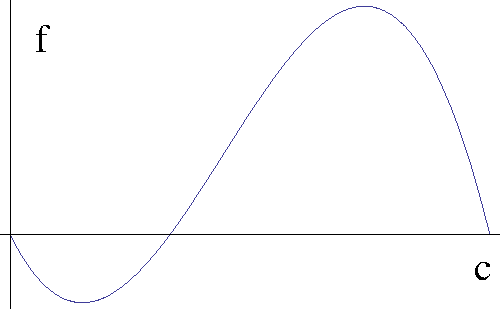
\includegraphics[width=0.5 \linewidth]{rysunki/rozdzial_3/f_PLOT.pdf} 
	\caption[Wykres autokatalitycznej funkcji źródłowej]{{\small Wykres autokatalitycznej funkcji źródłowej w równaniu (\ref{stand}). Po przekroczeniu pewnej wartości progowej $[Ca^{2+}]$ następuje autokatalityczny wypływ jonów wapnia z magazynów retikularnych. Takie zachowanie związane jest z własnościami kanałów retikularnych, których przewodnictwo zadane jest stanem receptorów IP$_3$/RyR.}}
    \label{f31}
\end{figure}

Oprócz kluczowego wpływu na inicjację wielu ścieżek sygnałowych wewnątrz komórki, podwyższone stężenie wolnych jonów wapniowych może generować naprężenia mechaniczne \cite{Murray2007}. Co więcej, zgodnie z klasycznymi prawami termodynamiki, zjawisko powyższe ma swoje lustrzane odbicie: mechaniczne naprężenia wewnątrz komórki lub na membranie komórkowej mogą być źródłem lokalnych zmian stężenia wolnych jonów wapniowych. 

\medskip 
W najprostszym modelu \cite{Murray2007} równania opisujące ewolucję stężenia jonów wapniowych oraz towarzyszące jej zjawiska mechaniczne w ośrodkach biologicznych (komórkach lub tkankach) mają następującą postać: 

\begin{equation} \label{1}
\frac{\partial c}{\partial t} = D_{eff} \nabla^2  c + 
f(c) + \gamma \theta, 
\end{equation}

\begin{equation}  \label{2} \nabla \cdot {\mbox{\boldmath$\sigma$}} = 0, \end{equation}

\bigskip 

\noindent gdzie $\theta = \nabla \cdot {\boldsymbol u}$ jest tzw. dylatacją a ${\boldsymbol u}$ jest wektorem przemieszczenia w punkcie. 
Tensor ciśnień {\mbox{\boldmath$\sigma$}}$\equiv \sigma_{ij}$, gdzie 

\begin{equation} \label{3}
\sigma_{ij} = \theta \lambda \delta_{ij} + 2 G \eps_{ij} + 
\nu_1 \theta_{,t} \delta_{ij} + \nu_2 \eps_{ij,t} + \tau_{ij}.  
\end{equation}

\noindent $\nu_1$ i $\nu_2$ są tutaj odpowiednimi współczynnikami lepkości ,,materiału'' komórki rozpatrywanej jako ośrodek mechaniczny. Jak poprzednio, w  równaniu (\ref{1}) $c$ oznacza stężenie wolnych jonów wapnia w cytozolu,  $D_{eff}$ dla jonów wapnia jest ich efektywnym współczynnikiem dyfuzji, $f(c)$ funkcją opisującą transport jonów wapniowych do- oraz z-~cytozolu (tzn. ich przepływ między cytozolem a pozostałymi kompartmentami oraz ewentualnie przestrzenią międzykomórkową). W równaniu (\ref{3}) $\eps_{ij}$ są składowymi tensora deformacji ${\boldsymbol \eps}=1/2 (\nabla {\boldsymbol u} + \nabla {\boldsymbol u}^T)$, $\lambda$ oraz $G$ oznaczają współczynniki Lame'a $\nu_1$ i~$\nu_2$ są współczynnikami lepkości. $\tau_{ij}$ są składowymi tzw. aktywnego tensora sił trakcji ${\boldsymbol \tau}$. Siły te związane są z oddziaływaniami aktyno-miozynowymi, dokładniej z~tworzeniem się mostków miozynowych pomiędzy włóknami aktynowymi prowadzącymi do kontrakcji ośrodka. Częstym założeniem nakładanym na tensor trakcji, które będzie przyjęte poniżej, jest jego diagonalność: 

\[ {\boldsymbol \tau} = {\mathrm diag}(\tau_{11},\tau_{22},\tau_{33}).\]

\noindent  W równaniu (\ref{2}), zostały pominięte człony inercjalne, tj. $\frac{\p \rho {\boldsymbol w} }{\p t} +  \frac{1}{2} \nabla \cdot ( \rho ~ {\boldsymbol w}\otimes {\boldsymbol w})$,gdzie $\rho$~jest (uśrednioną) gęstością ośrodka a $w$ jego lokalną prędkością, ponieważ towarzyszące dynamice wapniowej zjawiska mechaniczne indukują przemieszczenia punktów ośrodka odbywające się ze stosunkowo niewielkimi prędkościami. Poniżej, założymy również, że dywergencja tensora napięć jest równa zeru. Jest to równoważne założeniu, że nie ma żadnych zewnętrznych więzów na ekspansję lub też kontrakcję poszczególnych elementów ośrodka. (Z założenia tego zrezygnujemy w ostatnim rozważanym przez nas przypadku.) Liniowa forma członu mechanochemicznego ($\gamma \theta$) w równaniu została zapostulowana w książce \cite{Murray2007}, tom 2, równanie 6.72. 

\medskip 

Dynamika lokalnego stężenia wapnia wewnątrz komórki lub grupy komórek koordynuje szereg procesów fizjologicznych. Odgrywa kluczową rolę w przekazywaniu bodźców do wnętrza komórki oraz uczestniczy w procesie tworzenia się mostków miozynowych pomiędzy włóknami aktyno-miozynowymi. Proces ten jest szczególnie ważny w~długich komórkach mięśniowych, gdyż prowadzi do ich kontrakcji. Z drugiej strony, lokalne deformacje komórki, wpływają na dynamikę wapnia poprzez ich  mechaniczne oddziaływanie na wewnątrzkomórkowe magazyny wapniowe (głównie retikulum). Jak wspomnieliśmy, oddziaływanie to opisuje się za pomocą wyrażenia $\gamma \theta$. 

\medskip 

W pracy \cite{Kazmierczak2010} byliśmy zainteresowani dokładnymi rozwiązaniami w postaci fali biegnącej dla układu równań (\ref{1})-(\ref{3}). Tak więc, poszukiwaliśmy dokładnych (tj. zadanych jawnie) funkcji $c(x,y,z,t)$ oraz $\theta(x,y,z,t)$, $x,y,z \in \mathbb{R}$, $t \in \mathbb{R}$ spełniających warunek w postaci:  

\begin{equation} \label{ansatz}
c(x,y,z,t) = c(x-vt,y,z), \quad \theta(x,y,z,t) = \theta(x-vt,y,z)
\end{equation}

\noindent gdzie $v$ jest tutaj prędkością przesuwania się frontu falowego. Zakładamy zatem, że front ten propaguje się wzdłuż ustalonego kierunku, który dla uproszczenia utożsamiamy z osią $x$-ów. Zakładamy też, że asymptotycznie w $x$ (tzn. dla ustalonego $t$~i~$x \to \pm \infty$) wartości  $c(x,t)$ dążą do jednego ze stabilnych stanów równowagi (pierwsze i~trzecie miejsce zerowe na Ryc.~\ref{f31}). Ze względu na możliwość liniowego przeskalowania, bez straty ogólności, możemy założyć, że stany te odpowiadają wartościom  $c=0$ lub $c=1$.

\medskip 

Rozwiązania takie opisują sytuację, w której obszar podwyższonego stężenia wapnia rozszerza się z pewną stałą prędkością. Jednocześnie, stan naprężeń mechanicznych ośrodka również zmienia się w czasie i przestrzeni, podążając za zmieniającym się stężeniem wapnia. 

\medskip 

Dla bistabilnej funkcji źródłowej $f$ w postaci wielomianu trzeciego stopnia $A c(c-a)(1-c)$ dokładna postać dla czysto chemicznych fal biegnących stężenia wapnia (tzn. dla $\gamma=0$) jest dobrze znana. Natomiast, dokładne rozwiązania w postaci fal biegnących $c(x-vt), \quad \theta(x-vt)$, przy uwzględnieniu oddziaływania mechano-chemicznego i niezerowych (choć dostatecznie małych współczynników lepkości $\nu_1$ i $\nu_2$), nie zostały dotychczas znalezione.

\medskip 

\noindent\textbf{ Uwaga}
\begin{itemize}
\item Zakładając, że rozwiązanie ma postać fali biegnącej, dokonaliśmy matematycznej idealizacji problemu. Idealizacja taka jest usprawiedliwiona, jeśli rozpatrywane komórki możemy w istocie przybliżać poprzez bardzo długie i cienkie struktury cylindryczne z dobrze określoną ustaloną osią. 
Określenie 'bardzo długie' nakłada zarówno warunek na stosunek długości do liniowych wymiarów przekroju poprzecznego, jak i na stosunek szerokości frontu falowego do drogi jaką przebywa on w jednostkowym czasie. 
\item Przyjmując postać funkcji źródłowej w postaci $A c(c-a)(1-c)$, założyliśmy, że stężenie wapnia $c$ zostało liniowo przeskalowane tak, że poziom nieobudzony (stan spoczynkowy komórki) odpowiada wartości $c=0$, a poziom pobudzony wartości $c=1$ (aktywacja komórki). Powyższa bistabilna postać funkcji $f$ opisuje autokatalityczny wypływ jonów wapniowych z magazynów retikularnych. Zakładamy zatem, że lokalne podwyższenie stężenia jonów wapniowych w cytozolu powoduje wypływ wapnia z retikulum, jeśli przekracza ono pewien poziom krytyczny i ustaje, gdy osiąga pewną dostatecznie dużą wartość \cite{Keener2009} - Rozdz. 7.4.1, tom 2,\cite{Murray2007} - Rozdz.~6, tom 2. \B
\end{itemize}

\medskip 

W pracy \cite{Kazmierczak2010} znalezione zostały jawne rozwiązania w postaci fal biegnących dla układu (\ref{1})-(\ref{2}). Rozwiązania takie mogą dać nam pewien wgląd w makroskopowy charakter oddziaływań chemiczno-mechanicznych. Rozważania nasze przeprowadziliśmy w trzech przypadkach geometrycznych, pokazanych na Ryc.~\ref{f1}. Tak wiec, rozważyliśmy fale wapniowe w całej przestrzeni, cienkiej nieskończenie rozciągłej warstwie, która w swojej niezdeformowanej mechanicznie postaci jest płaszczyzną oraz nieskończenie długie struktury cylindryczne o dostatecznie małej średnicy modelujące długie komórki. Przypadki te zostały przeanalizowane również przy uwzględnieniu równań opisujących dynamikę białek buforujących w pracach \cite{Kazmierczak2013} oraz \cite{Kazmierczak2011}.

\medskip

Jak zauważyliśmy dynamika wapnia w komórce jest bardzo skomplikowanym zjawiskiem. Jony wapnia mogą być magazynowane nie tylko w ER, ale i innych organellach komórkowych (Tab.~\ref{tab:caakt}), w których związane są z wieloma ścieżkami sygnałowymi. W poszukiwaniu ścisłych postaci mechanochemicznych fal biegnących ograniczyliśmy się jedynie do procesów uwalniania wapnia z wewnątrzkomórkowych magazynów retikularnych do cytozolu. Zakładamy przy tym, że możemy zaniedbać niejednorodność przestrzenną rozmieszczenia struktur retikularnych oraz możliwy wpływ więzów mechanicznych wpływających na położenie komórki w przestrzeni, czy też elementów cytoszkieletu, utrzymujących swoisty typ kształtu komórki. 



\begin{figure} 
	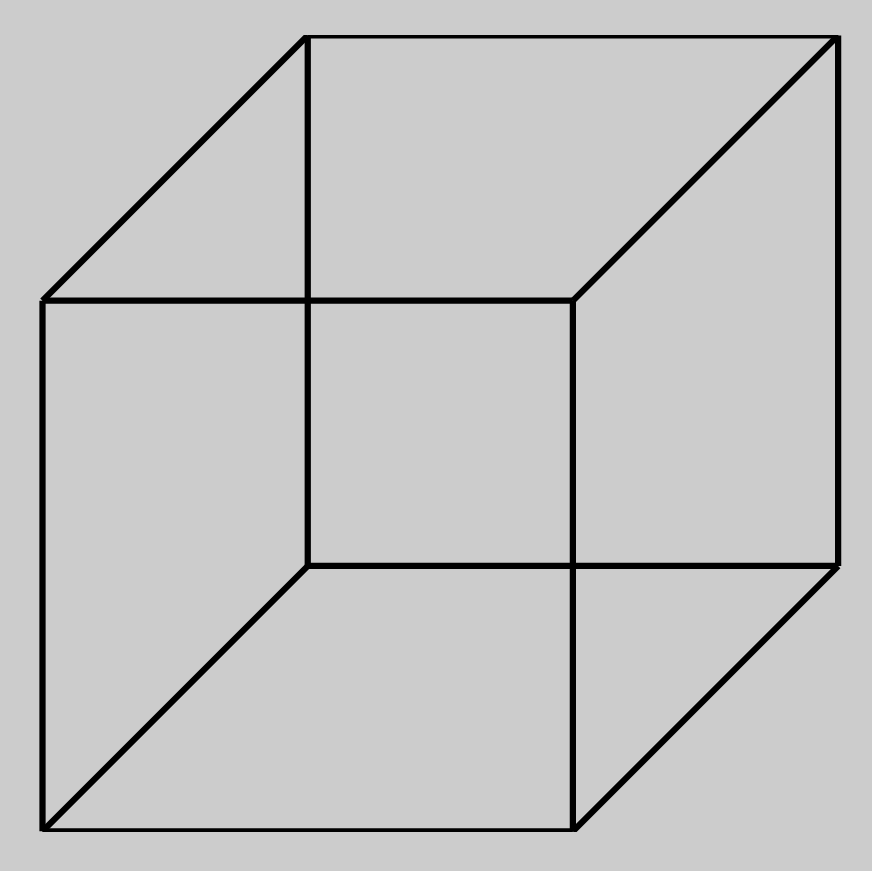
\includegraphics[width=0.243\linewidth]{rysunki/rozdzial_3/parap.png} 
	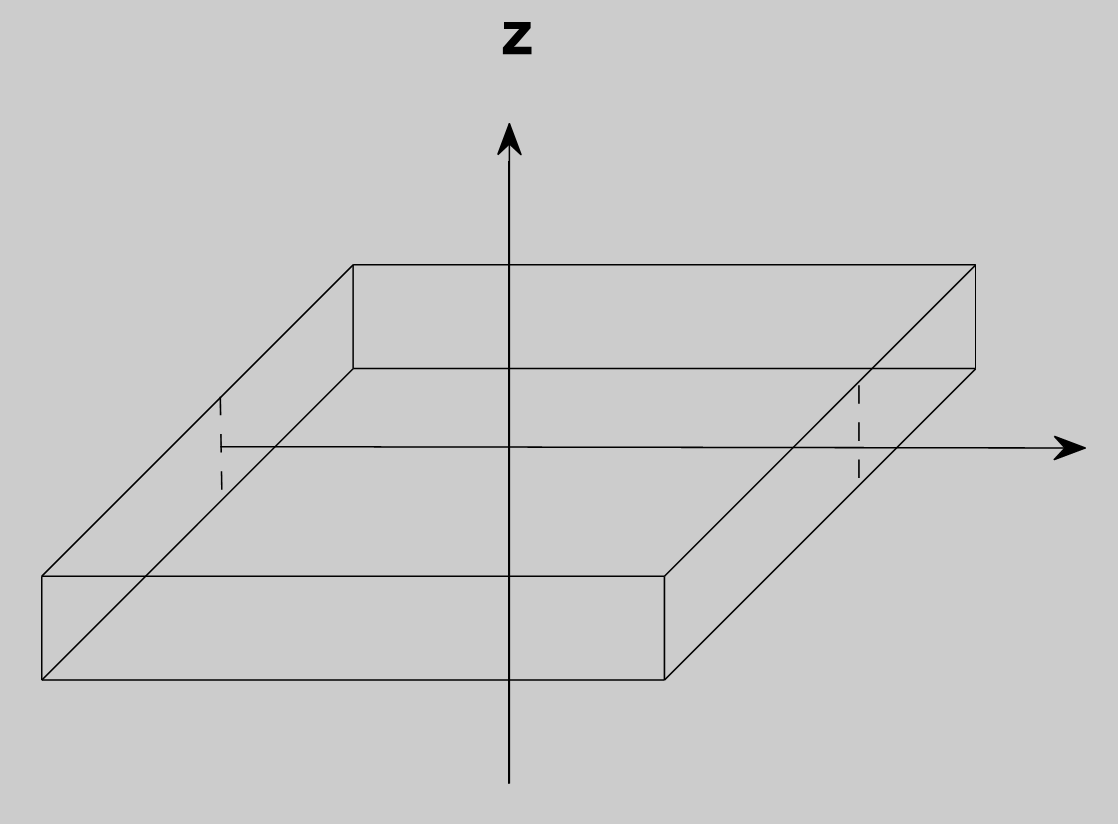
\includegraphics[width=0.33\linewidth]{rysunki/rozdzial_3/plate12.png} 
	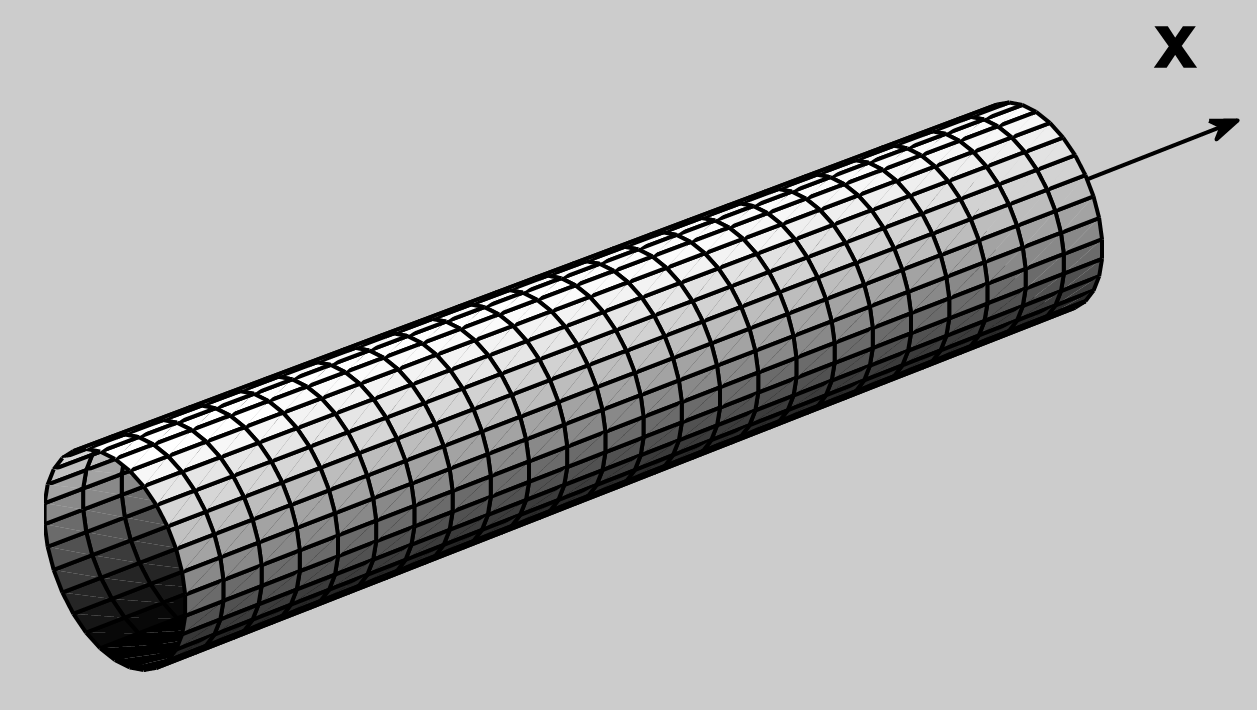
\includegraphics[width=0.43\linewidth]{rysunki/rozdzial_3/walec2.png} \\
	\caption[Struktury geometryczne rozważane w pracy]{Struktury geometryczne rozważane w pracy \cite{Kazmierczak2010}. Od lewej do prawej: a.~cała przestrzeń b. nieskończona płaska warstwa o dostatecznie małej grubości $2d$. c.~nieskończony cylinder o dostatecznie małym promieniu}\label{f1}
\end{figure}


\medskip 

\subsubsection{Analiza równania mechanicznego} \label{secmech} 

\medskip 

%Wykorzystując rozważania w pracach \cite{Peradzynski2014} or \cite{Kazmierczak2013} możemy, 
Poszukując rozwiązań w postaci fal biegnących (\ref{ansatz}), uprościliśmy układ równań różniczkowych cząstkowych (\ref{2})-(\ref{3}) opisujący efekty mechaniczne do jednego równania różniczkowego zwyczajnego postaci \cite{Kazmierczak2010,Kazmierczak2013,Kazmierczak2011}: 

\begin{equation} \label{mech1} 
K \theta + \mu \theta_{,t} + {\tau} =0. \qquad K, \mu, \tau  =const.
\end{equation}

\medskip 

\noindent Współczynniki $K$, $\mu$ oraz $\tau$ zależą od rozpatrywanego przypadku geometrycznego i są podane w Tab.~\ref{tab:tensor}. $\tau$ jest odpowiednią funkcją składowych tensora ${\boldsymbol \tau}$. 

\medskip

\begin{table}
	\centering
	\begin{tabular}{@{} | l |c | c | c | c | @{}}
		\hline 
		&&&& \\
		&$K(\lambda,G)$ & $K(E,\nu)$ &$\mu$& $\tau$ \\ 
		&&&& \\ \hline 
		&&&& \\
		\textsc{cała przestrzeń} & $\lambda+2G$ & $\frac{E(1-\nu)}{(1+\nu)(1-2\nu)}$ 
		& $\nu_1+\nu_2$ & $\tau_{11}$ \\ 
		&&&& \\
		\textsc{cienka warstwa} & $2\lambda+2G$ & $\frac{E}{(1+\nu)(1-2\nu)}$ &
		$2\nu_1+\nu_2$ & $\tau_{11}+\tau_{33}$ \\ 
		&&&& \\
		\textsc{włókno} & $3\lambda+2G$ & $\frac{E}{1-2\nu}$ & $3\nu_1 + \nu_2$ &
		$\tau_{11}+2\tau_{33}$ \\ 
		&&&& \\ 
		\hline
	\end{tabular}
	\caption[Współczynniki $K$, $\mu$ oraz $\tau$]{Współczynniki $K$, $\mu$, $\tau$ w równaniu (\ref{mech1}) dla rozpatrywanych geometrii}
	\label{tab:tensor}
\end{table}

\medskip 

W trzeciej kolumnie tabeli znajdują się wyrażenia wyrażające stałą $K$ poprzez częściej używane współczynniki mechaniczne, moduł Younga $E$ oraz współczynnik Poissona $\nu$. Zależności między $E$ i $\nu$ oraz $\lambda$ i $G$ są następujące: 

\[ \lambda =\frac{E\nu }{\left(1+\nu \right)(1-2\nu )}, ~ G =\frac{E}{2\left(1+\nu \right)} \]

\noindent oraz     


\[ E = \frac{G (2G +3\lambda )}{\lambda +G }, ~ \nu =\frac{\lambda }{2(\lambda +G )} \]  

\medskip 

\subsubsection{Fale biegnące}  \label{travel}

\medskip 

Oprócz założenia (\ref{ansatz}), przyjmiemy również, że lokalne przemieszczenie punktów ośrodka wywołane przez zmiany stężenia wapnia ma również postać fali biegnącej w~kierunku $x$

\begin{equation} \label{travu} 
\boldsymbol{u}(x,y,z,t) = \boldsymbol{u}(x-vt,y,z). 
\end{equation}

\noindent Dla rozwiązań w postaci fal biegnących układ (\ref{1})-(\ref{mech1}) przechodzi w układ zwyczajnych równań różniczkowych postaci:

\begin{equation} \label{c1} 
D c'' + v c' + f(c) + \gamma \theta = 0. 
\end{equation}

\begin{equation} \label{id3} 
-v \mu \theta' + K \theta + \tau = 0. 
\end{equation}

\noindent $'$ oznacza tutaj pochodną względem zmiennej falowej $\xi = x - vt$. Poszukujemy zatem rozwiązań heteroklinicznych układu (\ref{c1})-(\ref{id3}), tzn. funkcji $c$ oraz $\theta$ klasy $C^2$ spełniających warunki brzegowe w $\pm \infty$: $\lim_{\xi \to -\infty} c(\xi) = c_1$, $\lim_{\xi \to \infty} c(\xi) = c_3$ oraz $\lim_{|\xi| \to \infty} \theta(\xi) = 0$, gdzie $c_1$ i $c_3>c_1$ oznaczają stabilne stężenia jonów wapniowych w~cytozolu. Rozważając układ (\ref{1})-(\ref{2}), zakładamy również, że 

\begin{equation}  \tau(c_1)=\tau(c_3)=0, \quad {\mathrm oraz} \quad \tau(c) \geq 0. \end{equation} 

\noindent Jak sugerowaliśmy w punkcie drugim Uwag, poprzez zastosowanie liniowej transformacji zmiennej do $c$, możemy przyjąć bez straty ogólności, że 

\[  c_1=0, \quad c_3 = 1 \] 

% \noindent Poniżej przyjmiemy zatem, że funkcja źródłowa 

% \[ f(c)=A c(c-a)(1-c) \] 

\noindent Warunki brzegowe przyjmują wtedy postać

\[ \lim_{\xi \to -\infty} c(\xi) = 0, ~\lim_{\xi \to \infty} c(\xi) = 1, 
\quad  
\lim_{|\xi| \to \infty} \theta(\xi) = 0 \] 

\medskip 

Dla ustalenia uwagi ograniczymy się również do rozpatrywania sytuacji, w których obszar zajmowany przez wyższe stężenie rozszerza się z czasem. Tak więc, rozpatrujemy fale, których profil ma postać pokazaną na Ryc.~\ref{FM}. 


\begin{figure}[ht!]  
	\hspace{2cm} 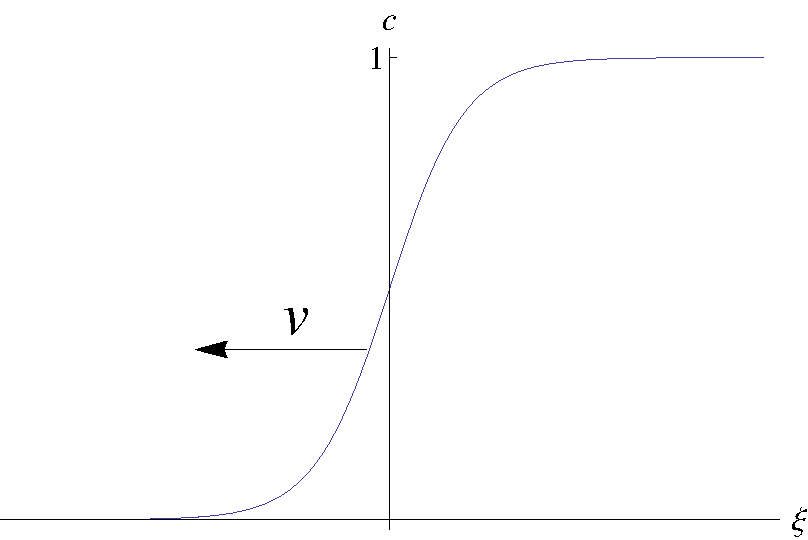
\includegraphics[width=0.85\linewidth]{rysunki/rozdzial_3/FALA_MICHAL.pdf} 
	\caption[Przykładowy profil fali biegnącej stężenia wapnia]{{\small Przykładowy profil fali biegnącej stężenia wapnia $c$. Fala porusza się w lewo z~prędkością $v$, przy czym profil zachowuje swój kształt w czasie. $\xi$ jest tutaj zmienną falową: $\xi = x - vt$. $v<0$, tak więc fala porusza się w lewo. }} \label{FM} 
\end{figure}

\noindent Z postaci (\ref{ansatz}) wynika, że pociąga to za sobą warunek $v<0$. Jeśli przyjąć, że 

\[ f(c)=A c(c-a)(1-c) \] 

\noindent to dla dostatecznie małych wartości funkcji opisujących sprzężenie mechano-chemiczne sytuacja taka będzie zagwarantowana warunkami: 

\begin{assum} \label{a0} 
	$(1-2 a) > 0$.
\end{assum}

\medskip 

\noindent Rozważania dotyczące 'fizycznych' wartości $A$ oraz efektywnych wartości współczynnika $D$ można znaleźć np. w \cite{Kazmierczak2011} oraz \cite{Keener2009} - Rozdz. 7.4.1, tom 2.  


\begin{assum} \label{a01} 
	Współczynniki $\gamma$, $\lambda$, $G$, $\nu_1$, $\nu_2$ 
	są stałymi, podczas gdy $\tau=\tau(c)$.
\end{assum}

\medskip 

\begin{assum} \label{a02} 
	Wartości współczynników lepkości $\nu_1$, $\nu_2$, a więc i współczynnika $\mu$ są dostatecznie małe.
\end{assum} 

\noindent \textbf{Uwaga dotycząca postaci funkcji $\tau(c)$} \\ \noindent Ponieważ nie jesteśmy w stanie znaleźć jawnych rozwiązań w przypadku ogólnym, postać ${\tau=\tau(c)}$ będzie dostosowana do postaci funkcji $\theta$. W zasadzie zależy ona od rodzaju komórek. $\tau=\tau(c)$ powinno być jednak dodatnie dla wszystkich niezerowych wartości $c$. W naszym rozważaniach przyjęliśmy, że $\tau=\tau(c)$ zachowuje się w przybliżeniu jak $c(1-c)$, a zatem że znika dla niskiego stężenia równowagowego przeskalowanego do wartości $c=0$ (lewy panel na Ryc.~\ref{fig2}). Rozważyliśmy również przypadek pokazany na prawym panelu Ryc.~\ref{fig2}, w którym $\tau(0)>0$. Takie postaci zgodne są z jakościową charakteryzacją funkcji trakcji np. w książce \cite{Murray2007} - Rozdz.~6, tom 2. 

\medskip

\begin{figure} 
	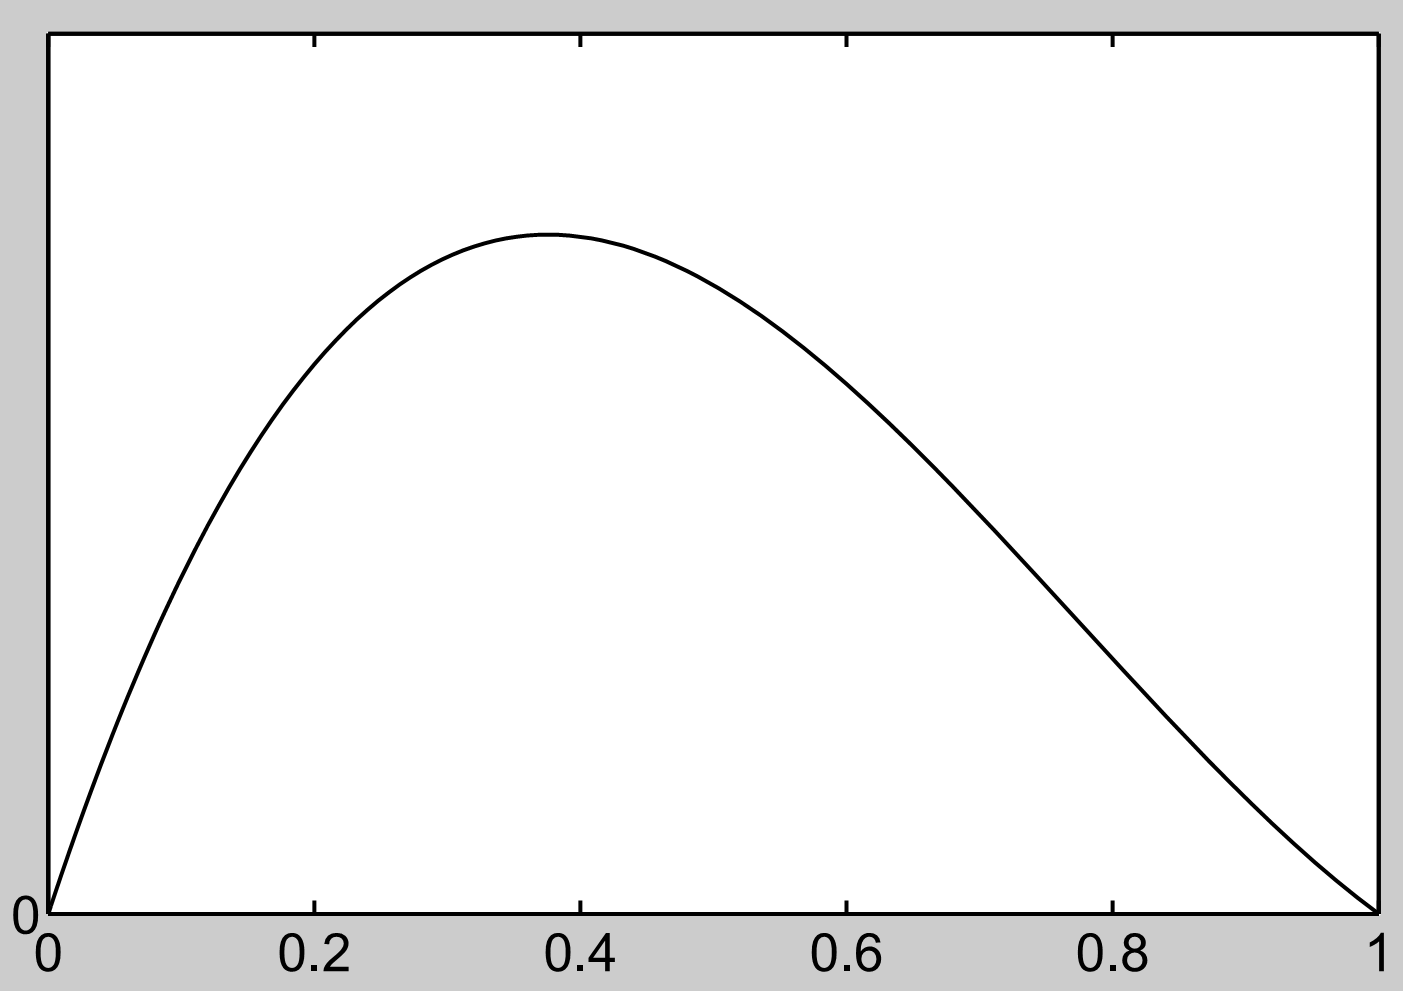
\includegraphics[width=0.49\linewidth]{rysunki/rozdzial_3/taumaj1.png} 
	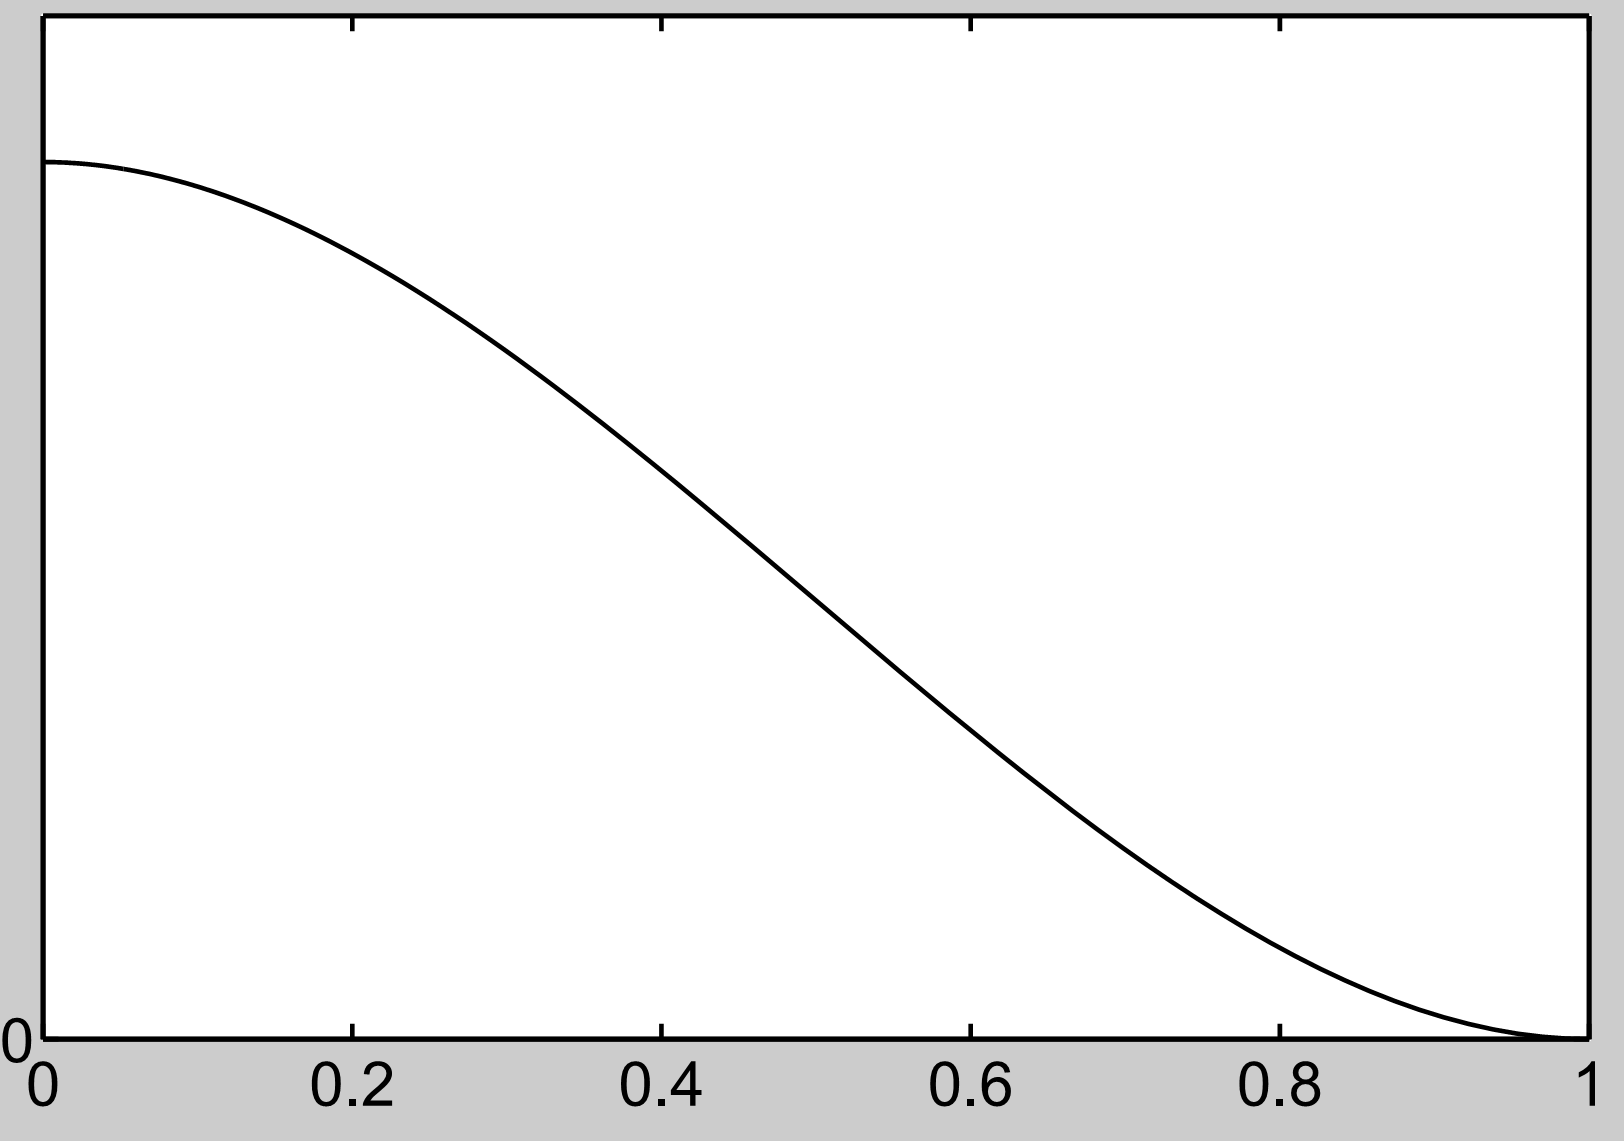
\includegraphics[width=0.493\linewidth]{rysunki/rozdzial_3/taumaj2.png} \\
	\caption[Postaci funkcji $\tau(c)$]{Postaci funkcji $\tau(c)$ dla $c \in [0,1]$.} \label{fig2}
\end{figure} 

Wiadomo, że dla $\theta = 0$, równanie (\ref{c1}) ma rozwiązanie heterokliniczne łączące jego stany stałe $c=0$ i $c=1$ dla dokładnie jednej wartości parametru $v$ równej: 

\[ v = - (AD/2)^{1/2} ( 1 - 2 a). \]

\noindent Rozwiązanie równania (\ref{c1}) ma postać: 

\[ c(\xi) = \frac{1}{1+\exp( -(\frac{A}{2D})^{1/2} \xi)}. \] 

\noindent Udowodnimy, że funkcja o podobnej strukturze, jest również rozwiązaniem układu (\ref{c1})-(\ref{id3}) uwzględniającego sprzężenie mechano-chemiczne. Załóżmy: 

\begin{equation} \label{ansatz2}
c = \frac{1}{1 + \exp(-s \xi)}, 
\end{equation} 

\noindent $s \geq 0$. Powyższa funkcja spełnia tożsamość: 

\begin{equation} \label{cprim} c' = s c(1-c) \end{equation}  

\noindent oraz $c(0)=1/2$. Załóżmy również, że 

\begin{equation} \label{thetac}  
\theta(\xi) = - q c(\xi)(1-c(\xi)) 
\end{equation} 

\noindent dla pewnego  $q \in IR^1$. Tak więc

\begin{equation} \label{thetaprim}  
\theta' = -s q c(1-c)(1-2c)  
\end{equation}

\noindent Wstawiając (\ref{thetac}) do równania (\ref{c1}) określającego profil fali, otrzymujemy:

\[ D c'' + v c' + Ac(c-a)(1-c) - \gamma q c (1-c) = 0 \]

\noindent i w konsekwencji

\[ D c'' + v c' + Ac(c-a + \gamma q A^{-1} )(1-c) = 0. \]

\noindent Powyższe równanie posiada rozwiązanie heterokliniczne 

\begin{equation} \label{prof} 
c(\xi) = \frac{1}{1+\exp( -(\frac{A}{2D})^{1/2} \xi)} 
\end{equation} 

\noindent spełniające warunek $c(0)=1/2$ \textbf{wtedy i tylko wtedy}, gdy  

\begin{equation} \label{speed} v = - (AD/2)^{1/2}\left( 1 - 2 (a + \gamma q A^{-1}) \right). \end{equation}

\noindent W szczególności, 
$\displaystyle{s= \sqrt{\frac{A}{2D}}}$. 
Zatem, zgodnie z (\ref{ansatz2}), (\ref{prof}) oraz (\ref{speed}), 

\begin{equation} \label{vs} 
vs= - \frac {A}{2}\left( 1 - 2 (a + \gamma q A^{-1}) \right). 
\end{equation} 

\begin{assum} \label{a02a} Załóżmy,że dla $\tau$ i $\mu$ zdefiniowanych w Tabeli 1, $\tau=\tau(c)$ spełniona jest tożsamość 
		
	\begin{equation} \label{id1p} 
	q c (1-c)\left[ K +  \frac A 2 \left( 1 - 2 (a + \gamma q A^{-1}) \right)  \mu (1-2c) \right] = \tau(c)   
	\end{equation} 
\end{assum} 

\noindent Zauważmy, że tożsamość (\ref{id1p}) może być spełniona, z uwagi na fakt, że, zgodnie z~Założeniem \ref{a02a}, wartość współczynnika $\mu$ jest mała. 

\medskip 

Zgodnie z (\ref{vs}), lewa strona wyrażenia (\ref{id1p}) może być zapisana w postaci \\\mbox{$q c (1-c)\left[ K -vs \mu (1-2c) \right]$}, tak więc Eq.(\ref{id3}) jest spełnione. 

\medskip 

W rezultacie naszych rozważań udowodniliśmy, że dokonując Założenia \ref{a02a} (zgodnego jakościowo z lewym panelem Ryc.~\ref{fig2} fala biegnąca $(c(\xi),\theta(\xi))$ o profilu $c$ danym przez (\ref{prof}) oraz profilu $\theta$ danym przez (\ref{thetac}), poruszająca się z prędkością (\ref{speed}) spełnia układ (\ref{c1})-(\ref{id3}). 

\medskip

\subsubsection{Lokalne przemieszczenia ośrodka}

\medskip

Dla uproszczenia ograniczymy się do ostatecznych wzorów na przemieszczenia \\$u_1(x,y,z,t)$ oraz $u_3(x,y,z,t)$ w przypadkach całej przestrzeni i nieskończonej cienkiej warstwy. Ich wyprowadzenie można znaleźć w pracy \cite{Kazmierczak2011}. W przypadku nieskończonego cylindra zamiast wzorów analitycznych przedstawimy przemieszczenia $u_1$ i $u_3$ (Ryc.~\ref{fig3} oraz Ryc.~\ref{fig4}). 
\medskip 

\noindent \textit{Cała przestrzeń}

\smallskip

% In this case we have $\boldsymbol{u} \equiv (u_1,0,0)$ 
% and $u_1(x,y,z,t) = \int_{-\infty}^\xi \theta(h) dh$, so 
% demanding that 
% $u_1 \to 0$ for $x-vt \to -\infty$, we have according to (\ref{thetaprim}): 

\[  u_1(x,y,z,t) = - q c(x,y,z,t) \sqrt{\frac{2D}{A}} \quad u_3 \equiv 0 \] 

\medskip  

\noindent \textit{Nieskończona cienka warstwa}

\smallskip


\[ u_1(x,y,z,t) = - q c(\xi)\sqrt{\frac{D}{2A}} 
\left[ 1 - A  \frac{\nu_2}{2G} ( 1 - 2 (a + \gamma q A^{-1}) ) (1-c(\xi)) 
\right] 
\]

\[
{\displaystyle 
	u_3(x,y,z,t) = - q c(\xi) (1-c(\xi)) \left[ \frac 1 2 +   \frac{A}{2G} 
	( 1 - 2 (a + \gamma q) ) \frac{\nu_2}{2} (1-2c(\xi)) \right] z}
\]
\medskip 

\noindent \textit{Nieskończony cylinder}

\medskip 

Jakościowe zachowanie się przemieszczeń $u_1$ i $u_3$ od współrzędnych $\xi$ oraz $z$, dla ustalonej chwili czasu $t$, przedstawione jest na Ryc.(\ref{fig3}) oraz Ryc.(\ref{fig4}).


\medskip 

\vspace{0cm}

\begin{figure}[ht!] 
	\centering 
	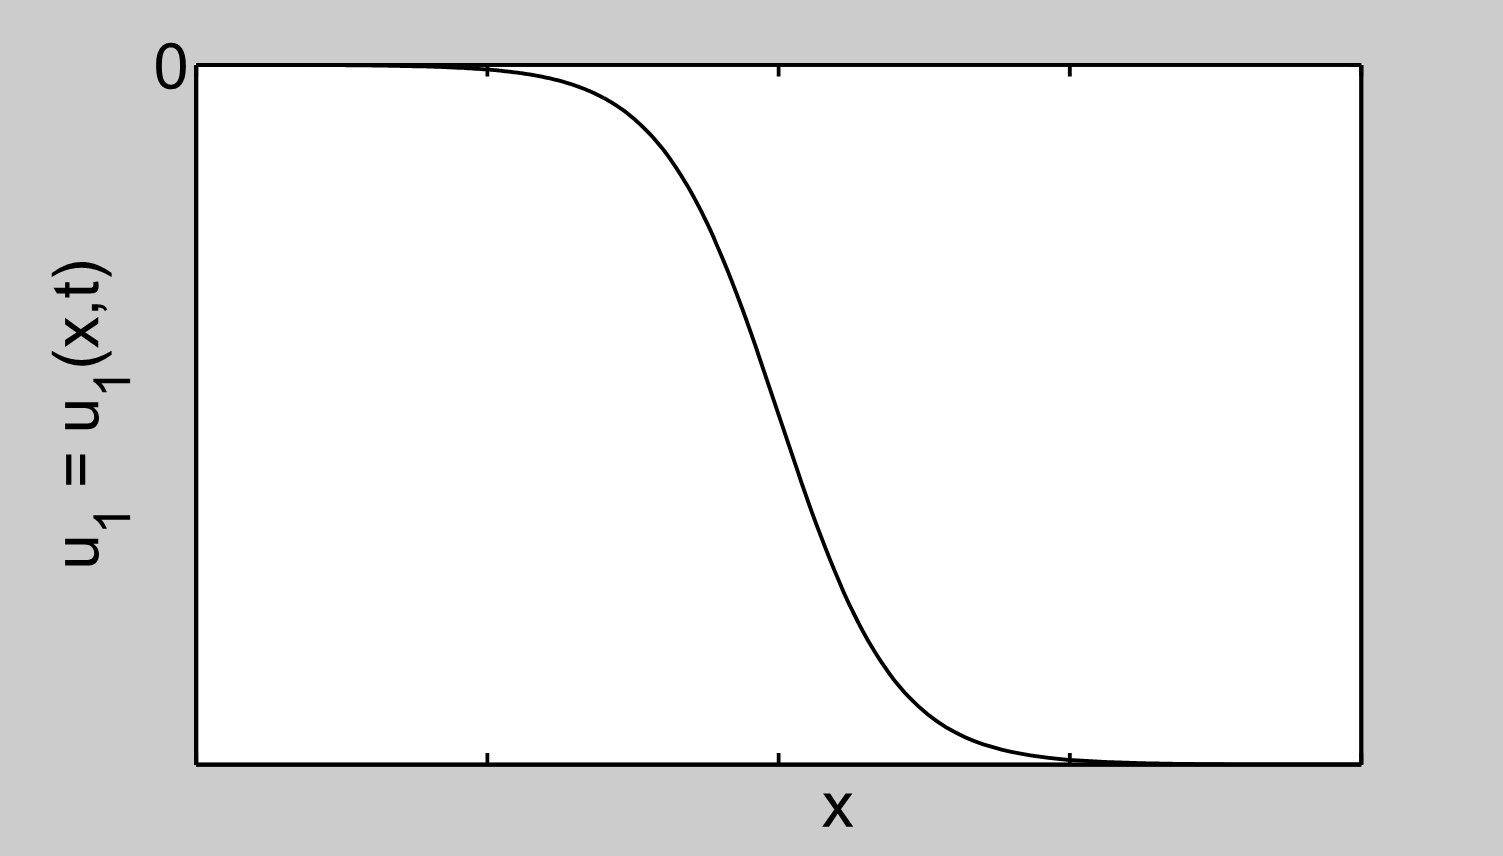
\includegraphics[width=1\linewidth]{rysunki/rozdzial_3/ku22L.png} \\ 
	\caption[Przemieszczenia w kierunku $x$]{Przemieszczenia w kierunku $x$. Wektory przemieszczenia $u_1(x,t)$ są skierowane w lewo. $u_1(x,t) \to 0$ jeśli $x \to -\infty$ oraz 
		$u_1(x,t) \to u_{10} < 0$ jeśli $x \to \infty$.} \label{fig3}
\end{figure}

\begin{figure}[h]
	\centering 
	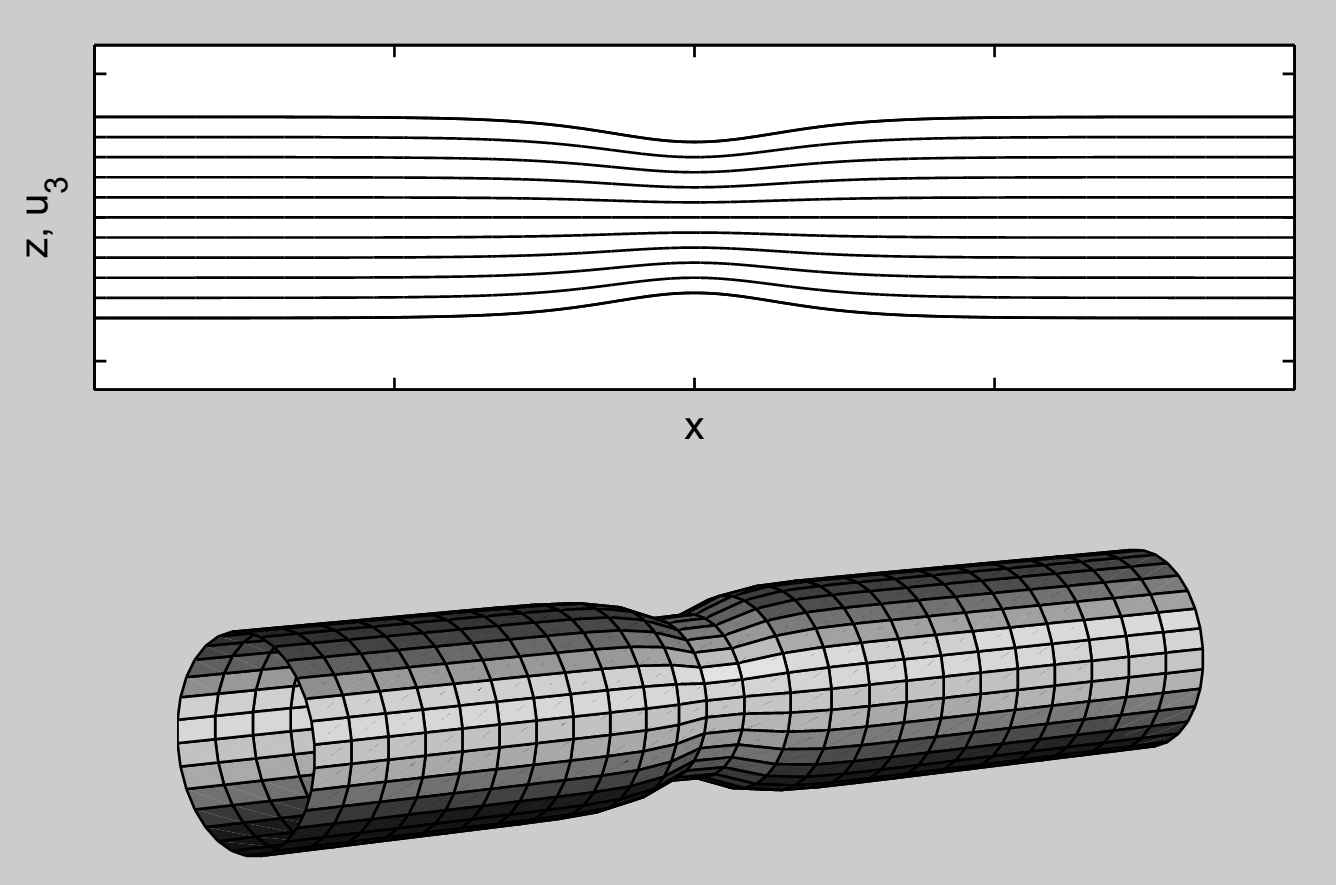
\includegraphics[width=1\linewidth]{rysunki/rozdzial_3/uzmech.png} \\
	\caption[Przemieszczenia w kierunku $z$]{Przemieszczenia w kierunku $z$. Górny panel: cienka warstwa. Dolny panel: długi cylinder.}
	\label{fig4}
\end{figure} 

\medskip 

\noindent Podaliśmy zatem szkic następującego twierdzenia: 

\begin{thm} 
	Niech spełnione będą założenia (\ref{a0}), (\ref{a01}), (\ref{a02}). Wtedy	dla wszystkich $q>0$, układ (\ref{c1}),(\ref{id3}) ma rozwiązanie heterokliniczne $(v,c,\theta)$, gdzie $v$ określone jest równaniem (\ref{speed}), $c(\xi)$ równaniem (\ref{prof}) a $\theta(\xi)$ zależnością (\ref{thetac}). Rozwiązanie jest jednoznacznie określone z dokładnością do translacji funkcji $c$ w kierunku osi $\xi$. \B
\end{thm}

\noindent Szczegóły dowodu można znaleźć w pracy \cite{Kazmierczak2010}.

\medskip 

\subsubsection{Mechanochemiczne fale biegnące z więzami mechanicznymi}

\medskip 

W pracy \cite{Kazmierczak2011} rozważono również istnienie i własności fal biegnących dla układu równań: 

\begin{equation} \label{11}
\frac{\partial c}{\partial t} = D_c \nabla^2 c + 
f(c) + \gamma \theta, 
\end{equation}

\begin{equation} \label{21} \nabla \cdot {\mbox{\boldmath$\sigma$}} = k {\boldsymbol u},
\end{equation}

\noindent gdzie $k = {\mathrm const}>0$. Tak więc w podejściu tym uwzględniamy możliwość istnienia więzów mechanicznych przeciwdziałających ruchowi punktów ośrodka. Specyficzna forma takich więzów, dana prawą stroną równania (\ref{21}), implikowana jest tzw. modelem Winklera. Dla ustalenia uwagi i prostoty rozważań skoncentrowaliśmy się na przypadku całej przestrzeni. Wykorzystując jawną postać rozwiązania w formie (\ref{ansatz2}), poszukiwaliśmy rozwiązania rozpatrywanego układu poprzez odpowiedni dobór funkcji $\tau(c)$. Analiza składowych tensora $\eps_{ij}$ w tym przypadku doprowadza nas do następujących relacji: 

\[ \theta=\eps_{11}, \quad {\boldsymbol u} = (u_1,0,0)=:(u,0,0) \]

\noindent skąd wynika, że 

\[ \theta = u_{,x} =u', \]

\noindent gdzie $'$ oznacza różniczkowanie względem zmiennej $\xi=x - vt$. W przeciwieństwie jednak do analizowanego powyżej przypadku, w którym $\nabla \cdot {\mbox{\boldmath$\sigma$}} = 0$, zakładamy, że $u(\xi) \to 0$ dla $\xi \to \pm \infty$ żądając, aby

\[ u(\xi) = -\zeta c'(\xi), \]

\noindent gdzie $\zeta = const$. Wynika stąd, że $\theta(\xi) = u'(\xi) = -\zeta c''(\xi)$. Na podstawie (\ref{ansatz2}) wynika, że 

\begin{equation} \label{t21} 
\theta = -s \zeta c(1-c)(1-2c). 
\end{equation} 

\noindent Tak więc na podstawie równania (\ref{cprim}) $\theta'$ jest wielomianem czwartego stopnia względem $c$ znikającym dla $c=0$ i $c=1$. Równanie (\ref{21}) może być zatem zapisane w~postaci 

\begin{equation} 
v \mu \theta' + K s \zeta c(1-c)(1-2c) - k \zeta c + \eta = \tau(c).
\end{equation}

\noindent gdzie $\eta$ jest stałą całkowania.